\chapter{Trabalhos Relacionados}
\label{trabalhos}

Como forma de elencar soluções e trabalhos relacionados ao desta pesquisa, alguns trabalhos, em conjunto com outros identificados no processo descrito na Seção \ref{fundamentacao:ageis:fatores},foram investigados. Esses trabalhos abordam a importância de garantir a alta qualidade do TE e propõe métodos de avaliar essa qualidade.

Em \cite{moe}, os autores propõem uma ferramenta que, segundo eles, contempla aspectos e características essenciais, apresentados em cinco dimensões (i.e., Liderança Compartilhada, Orientação da Equipe, Redundância, Aprendizagem da Equipe e Autonomia da Equipe) que precisam ser abordadas para garantir a alta qualidade do TE. Os conceitos dessas dimensões estão apresentados na Tabela \ref{fundamentacao:ageis:fatores:tabela}. Os resultados do instrumento são apresentados em um gráfico de radar, que representa o status atual do TE. Como forma de avaliar a qualidade do TE, foi definida uma pergunta pra cada dimensão abordada pela ferramenta. As perguntas devem ser respondidas em uma escala que vai de 0 à 10, onde os limites dessa escala são descritos para facilitar a resposta dessas perguntas por parte dos usuários. Essa ferramenta também é utilizada em \cite{ringstad}.

De acordo com os autores, pesquisadores e pessoas que atuam na indústria reconhecem que as cinco dimensões abordadas pela ferramenta são essenciais para o TE em ambientes ágeis. Além disso, a ferramenta é apropriada para verificar mudanças na qualidade do TE ao longo do tempo. Entretanto, essa abordagem não considera outros fatores essenciais que influenciam a qualidade do TE. Além disso, o gráfico de radar que contém o status atual do TE não provê informações objetivas acerca do estado atual do TE.

Hoegl et al. \cite{hoegl} conceitualizam a qualidade do TE como a qualidade das interações entre os membros de um time. Os autores propõem seis características indicadoras de colaboração no trabalho e as combinam como fatores determinantes para a qualidade do TE. Essas seis características são: Comunicação, Coordenação, Balanço da Contribuição dos Membros, Suporte Mútuo, Esforço e Coesão.

Nesse trabalho, a principal proposição dos autores é a de que a qualidade do TE está positivamente relacionada com o sucesso de projetos inovadores. Foram realizadas entrevistas com o intuito de coletar dados de equipes de desenvolvimento, gerentes de projeto e gerentes que não são parte da equipe para avaliar a veracidade dessa proposição. Nessas entrevistas, os indivíduos responderam perguntas relacionadas aos seis fatores que influenciam a qualidade do TE, e deram suas opiniões à respeito do sucesso de seus projetos. Com base nos resultados, os autores concluíram que o desempenho da equipe é positivamente influenciado pela qualidade do TE.

Entretanto, o conceito de qualidade do TE atrelado aos seis fatores descritos por Hoegl et al. \cite{hoegl} correspondem apenas ao grau colaboração da equipe, não contemplando fatores como, por exemplo, \textit{Autonomia da Equipe}. Além disso, apesar do contexto de projetos inovadores ser similar ao de projetos ágeis \cite{freire}, em \cite{hoegl} não há informações relacionadas às metodologias utilizadas nos projetos em que os indivíduos entrevistados trabalham.

\section{Trabalho Base}
\label{trabalhos:base}

Esta pesquisa tem como base o trabalho apresentado em \cite{freire}. Nesse trabalho, a necessidade de avaliar a qualidade do TE é apresentada, e um modelo baseado em \textit{Redes Bayesianas} é proposto para realizar essa avaliação. O conceito de qualidade do TE, nesse trabalho, é considerado como a união da eficiência da colaboração, do gerenciamento das atividades e dos atributos da equipe - atributos pessoais dos membros da equipe e o expertise deles.

O modelo proposto em \cite{freire} foi construído tomando como base apenas o trabalho de Hoegl et al. \cite{hoegl}. As modificações feitas no modelo base foram feitas com ajuda de especialistas em entrevistas separadas. Após as modificações, a versão final do modelo proposto ficou como representado na Figura \ref{trabalho:base:modelo}.

\begin{figure}[ht!]
\begin{center}
        \fbox{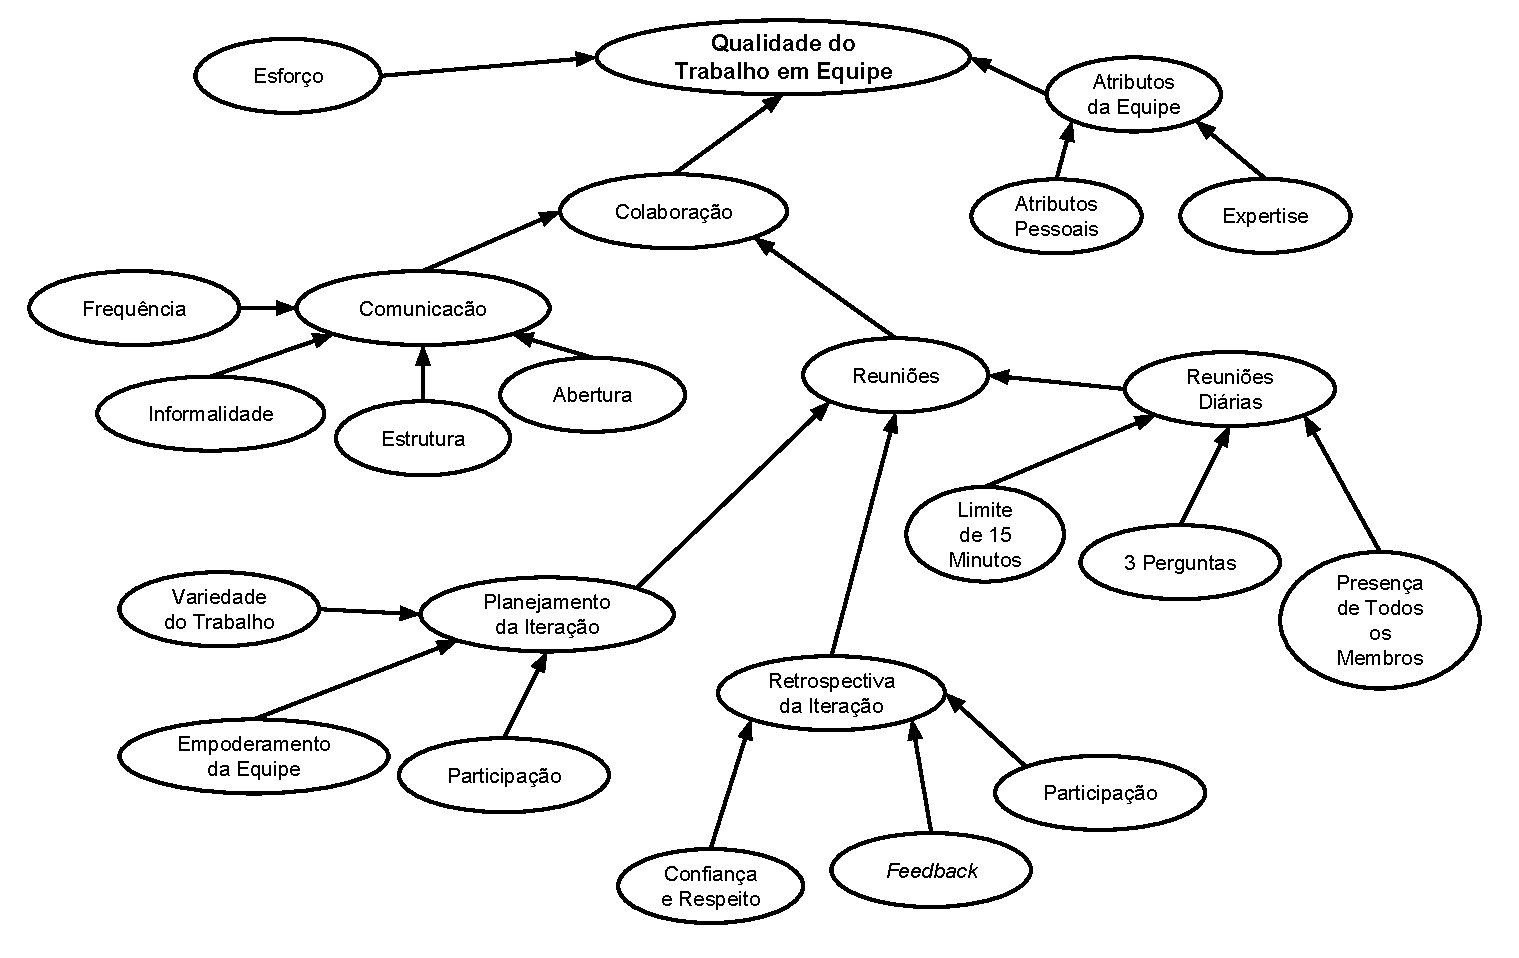
\includegraphics[scale=0.6]{figs/modeloSBES.pdf}}
    \end{center}
    \caption{Modelo Proposto no Trabalho Base}
    \label{trabalho:base:modelo}
\end{figure}

As tabelas de probabilidade desse modelo foram definidas utilizando o método de \cite{perkusichNPT}. Contudo, em vez de utilizar \textit{surveys} online, foram realizadas entrevistas com o mesmos especialistas responsáveis por construir o GAD. Para cada nó filho presente no GAD, pediu-se que os especialistas ordenassem seus nós pai com base na sua relevância para o nó filho. Em seguida, com base nessas ordens de relevância foram definidas as expressões ponderadas para, finalmente, definir as TPN dos nós filho.

A validação desse modelo foi feita com simulação de cenários, e, de acordo com as conclusões, o modelo é uma boa representação do mundo real. Além disso, também foi concluído que o modelo permite que, baseado nos resultados do modelo, os indivíduos que o utilizam identifiquem problemas que compromentem a qualidade do TE. Entretanto, há alguns fatores que afetam a sua validade. São eles:

\begin{itemize}
  \item A utilização de apenas um trabalho como base para o modelo;
  \item A definição das TPN utilizando o método de Perkusich et al. utiliza apenas a função de média ponderada. Logo, as TPN de alguns nós podem estar inconsistentes pelo fato de sua definição ser restrita à essa função;
  \item O modelo não validado em projetos reais.
\end{itemize}

Portanto, nesta pesquisa, foi dada continuidade no trabalho apresentado em \cite{freire}, buscando eliminar esses fatores que ameaçaram a sua validade.
